\chapter{Dise\~no del modelo el\'astico}
\label{cap:disenoSistema}

En este cap\'itulo se aborda el an\'alisis del modelo el\'astico de replicaci\'on de operadores de un SPS, tomando en consideraci\'on una t\'ecnica utilizada para el balance de carga, como tambi\'en las bases te\'oricas para el modelo dise\~nado. Adem\'as de lo anterior, se hace una descripci\'on detallada del dise\~no de cada uno de los m\'odulos del modelo.

\section{An\'alisis del m\'odelo el\'astico}
Dentro del an\'alisis realizado en la arquitectura del sistema implementado, se utiliza una perspectiva basada en los recursos l\'ogicos del sistema seg\'un el enfoque din\'amico, la cual es explicada en la Secci\'on \ref{subsec:recLogicosBC}, para el balance de carga del SPS. El presente trabajo no se enfoca en el an\'alisis del comportamiento de cada uno de los nodos f\'isicos del sistema, sino m\'as bien en el estado de cada uno de los operadores del grafo dise\~nado, siendo un problema de car\'acter l\'ogico y no f\'isico.

Respecto al estudio de las distintas t\'ecnicas implementadas, es necesario utilizar una que minimice la p\'erdida de datos, que sea capaz de adaptarse a las condiciones din\'amicas del tr\'afico, y que sea de bajo \textit{overhead} para el sistema, de tal manera que sea escalable. Bajo estas restricciones, se considera que la mejor opci\'on es utilizar la t\'ecnica de fisi\'on, utilizando el modelo de replicaci\'on de \citep{FernandezMKP13}, donde bas\'andose en el nivel de carga del operador, se eval\'ua la generaci\'on de una r\'eplica para \'este. \normalsize{Dentro de los supuestos realizados}, se plantea que el costo de un operador es menor a la formaci\'on de las colas de datos en el sistema, lo cual puede variar seg\'un la arquitectura del SPS implementando.

En la Figura \ref{fig:ejReplicacion} se muestra un ejemplo de la replicaci\'on propuesta. La Figura \ref{fig:ejReplicacion} (a) se presentan tres operadores, donde en el operador B existe una sobrecarga representada por una doble circunferencia, por lo que es necesario replicar el operador. En la Figura \ref{fig:ejReplicacion} (b) se presenta el mismo operador ya replicado, pero todav\'ia persiste la sobrecarga en \'este, por lo que se vuelve a realizar el mismo procedimiento, hasta que finalmente converge a la cantidad \'optima de r\'eplicas deseadas en el sistema en el per\'iodo de tiempo analizado, como se muestra en la Figura \ref{fig:ejReplicacion} (c).

\begin{figure}[!ht]
	\centering
		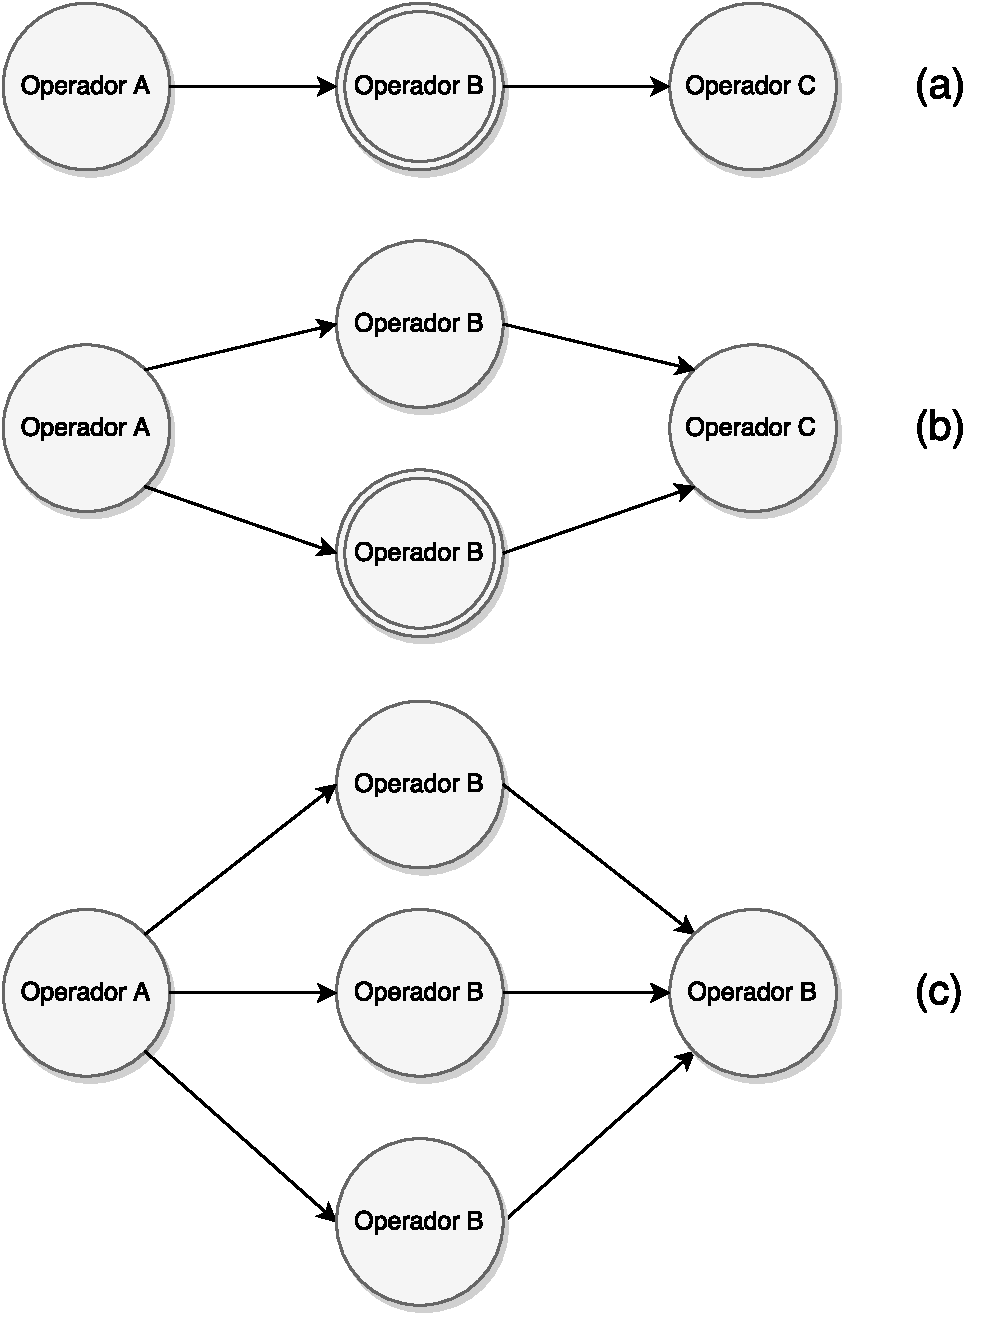
\includegraphics[scale=0.6]{images/EjReplicacion.pdf}
	\caption[Ejemplo de replicaci\'on del modelo propuesto.]{Ejemplo de replicaci\'on del modelo propuesto.\\Fuente: Elaboraci\'on propia.}
	\label{fig:ejReplicacion}
\end{figure}

%Para el dise\~no del sistema, era necesario contar con un umbral que determinara cuando el operador est\'a o no sobrecargado, por lo que para esto se utilizaron conceptos de teor\'ia de colas \citep{bose2013introduction}. Como los SPS est\'an orientados en grafos, se posee tanto la tasa de llegada ($\lambda$) como la tasa de procesamiento ($\mu$) para cada uno de los operadores, como se ve representando en la Figura \ref{fig:analisisTeoriaColas}, donde la tasa de procesamiento de un operador es la misma tasa de llegada del siguiente operador en el grafo. Utilizando este tipo de conceptos, para cada operador se calcul\'o la tasa de procesamiento ($\rho$), la cual esta definida por la tasa de llegada, la tasa de procesamiento y la cantidad de servicios disponibles en el sistema ($\rho = \frac{\lambda}{\mu \rho}$), cuyo valor nos indica el rendimiento del operador en cierta per\'iodo de tiempo.

Para la detecci\'on del nivel de carga de un operador es necesario contar con un modelo basado en umbrales que permita determinar cuando est\'a o no sobrecargado un operador. Para modelar esta situaci\'on se utilizan conceptos de teor\'ia de colas \citep{bose2013introduction}. Dado que los SPS utilizan un paradigma orientado a grafos, se puede obtener tanto la tasa de llegada ($\lambda$) como la tasa de procesamiento ($\mu$) de cada uno de los operadores que lo componen, como se ve representando en la Figura \ref{fig:analisisTeoriaColas}. Aqu\'i la tasa de procesamiento de un operador influye directamente en la tasa de llegada del siguiente operador en el grafo. Al utilizar estos conceptos, se calcula la tasa de rendimiento ($\rho$), la cual est\'a definida por la tasa de llegada, de procesamiento y la cantidad de r\'eplicas del operador, como se muestra en la Ecuaci\'on \ref{eq:tasaRendimiento}, cuyo valor representa el factor de utilizaci\'on del sistema, donde se define un sistema estable si y s\'olo si $\rho < 1$.

\begin{equation} \label{eq:tasaRendimiento}
	\rho = \frac{\lambda}{s \mu}
\end{equation}

\begin{figure}[!ht]
	\centering
	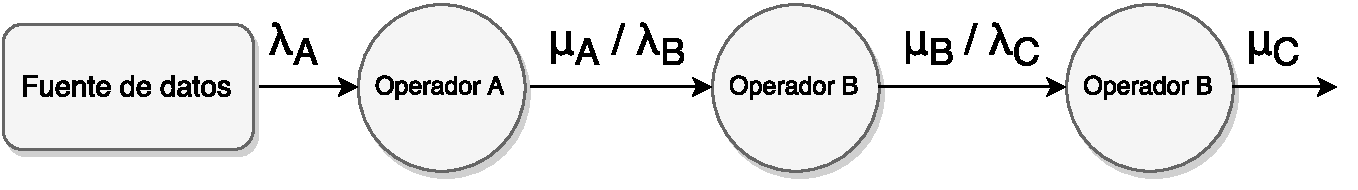
\includegraphics[scale=0.6]{images/AnalisisTeoriaColas.pdf}
	\caption[Enfoque de un SPS con conceptos de teor\'ia de colas.]{Enfoque de un SPS con conceptos de teor\'ia de colas.\\Fuente: Elaboraci\'on propia.}
	\label{fig:analisisTeoriaColas}
\end{figure}

Tomando en consideraci\'on el enfoque din\'amico en el algoritmo de balance de carga y la elasticidad que se pretende por parte del modelo, es que se han tratado tres posibles estados en el sistema: ocioso, estable e inestable. El primer estado corresponde a un exceso en la cantidad de recursos asignados. El segundo est\'a definido por el rendimiento \'optimo del sistema. Y por \'ultimo, el tercero hace referencia a un sistema sobrecargado, donde es necesario una mayor cantidad de recursos por parte de \'este. Los posibles estados de cada operador son la base para el an\'alisis y predicci\'on de la carga del modelo propuesto.

Para el modelo se consideraron dos tipos de algoritmos: predictivo, enfocado en el futuro basado en la historia del operador, y reactivo, analizando el comportamiento del momento. Este dise\~no tiene la finalidad de analizar dos factores: los \textit{peaks} existentes en la historia del operador, dado el algoritmo predictivo, y analizar el comportamiento en el momento, haciendo uso del algoritmo reactivo, de tal manera de solucionar los comportamientos que no son detectados con la predicci\'on.

%Es importante denotar que dependiendo del tipo de caso es que un algoritmo va a funcionar mejor. Por ejemplo, si existe una variaci\'on muy alta en un per\'iodo de tiempo considerable, el algoritmo predictivo puede detectar este tipo de \textit{peaks}. De esta manera, la predicci\'on es m\'as asertiva que el an\'alisis en el momento. Pero en casos que no suceda lo anterior, y s\'olo hayan variaciones en ciertos instantes de la ejecuci\'on, se encuentra el algoritmo reactivo para analizar el estado del operador.

\normalsize{Otra de las consideraciones realizadas es que cada uno de los algoritmos va a resolver un problema en espec\'ifico seg\'un su pol\'itica de resoluci\'on. Por ejemplo, si se desea detectar un comportamiento seg\'un el historial, el m\'as indicado es el algoritmo predictivo. Y en caso de analizar \textit{peaks} seg\'un el presente, el algoritmo reactivo puede dar soluciones al respecto.}

Adem\'as de lo anterior, se considera que es necesario trabajar con los dos algoritmos en temporalidades distintas, es decir, en cierto per\'iodo de tiempo se utiliza el reactivo y en otro el predictivo. Esto quiere decir que mientras se obtienen las $n$ muestras para realizar el c\'alculo de predictivo, el algoritmo reactivo est\'a realizando un an\'alisis de los distintos operadores.

%Al dise\~nar un sistema que pudiera lidiar con dos tipos de algoritmos, era necesario considerar un algoritmo que pudiera administrar la cantidad de cargas, con tal utilizar el algoritmo necesario seg\'un el per\'iodo existente en una ventana de tiempo, como tambi\'en la cantidad de r\'eplicas que deben aplicarse.

Como se dise\~naron dos tipos de algoritmos que se complementan, es necesario considerar un mecanismo que administre cual de los dos algoritmos se va a utilizar seg\'un el per\'iodo analizado, como tambi\'en la cantidad de r\'eplicas que deben crearse o eliminar seg\'un el resultado del algoritmo utilizado.

Dado lo anterior, se ha dise\~nado un modelo el\'astico \normalsize{basado en el modelo MAPE}\citep{redbooks2004practical}\normalsize{, el cual posea cuatro componentes}: monitor de carga, analizador de carga, predictor de carga y administrador de r\'eplicas, que se presenta en la Figura \ref{fig:componentesSistemas}.

\begin{figure}[ht!]
  \centering
    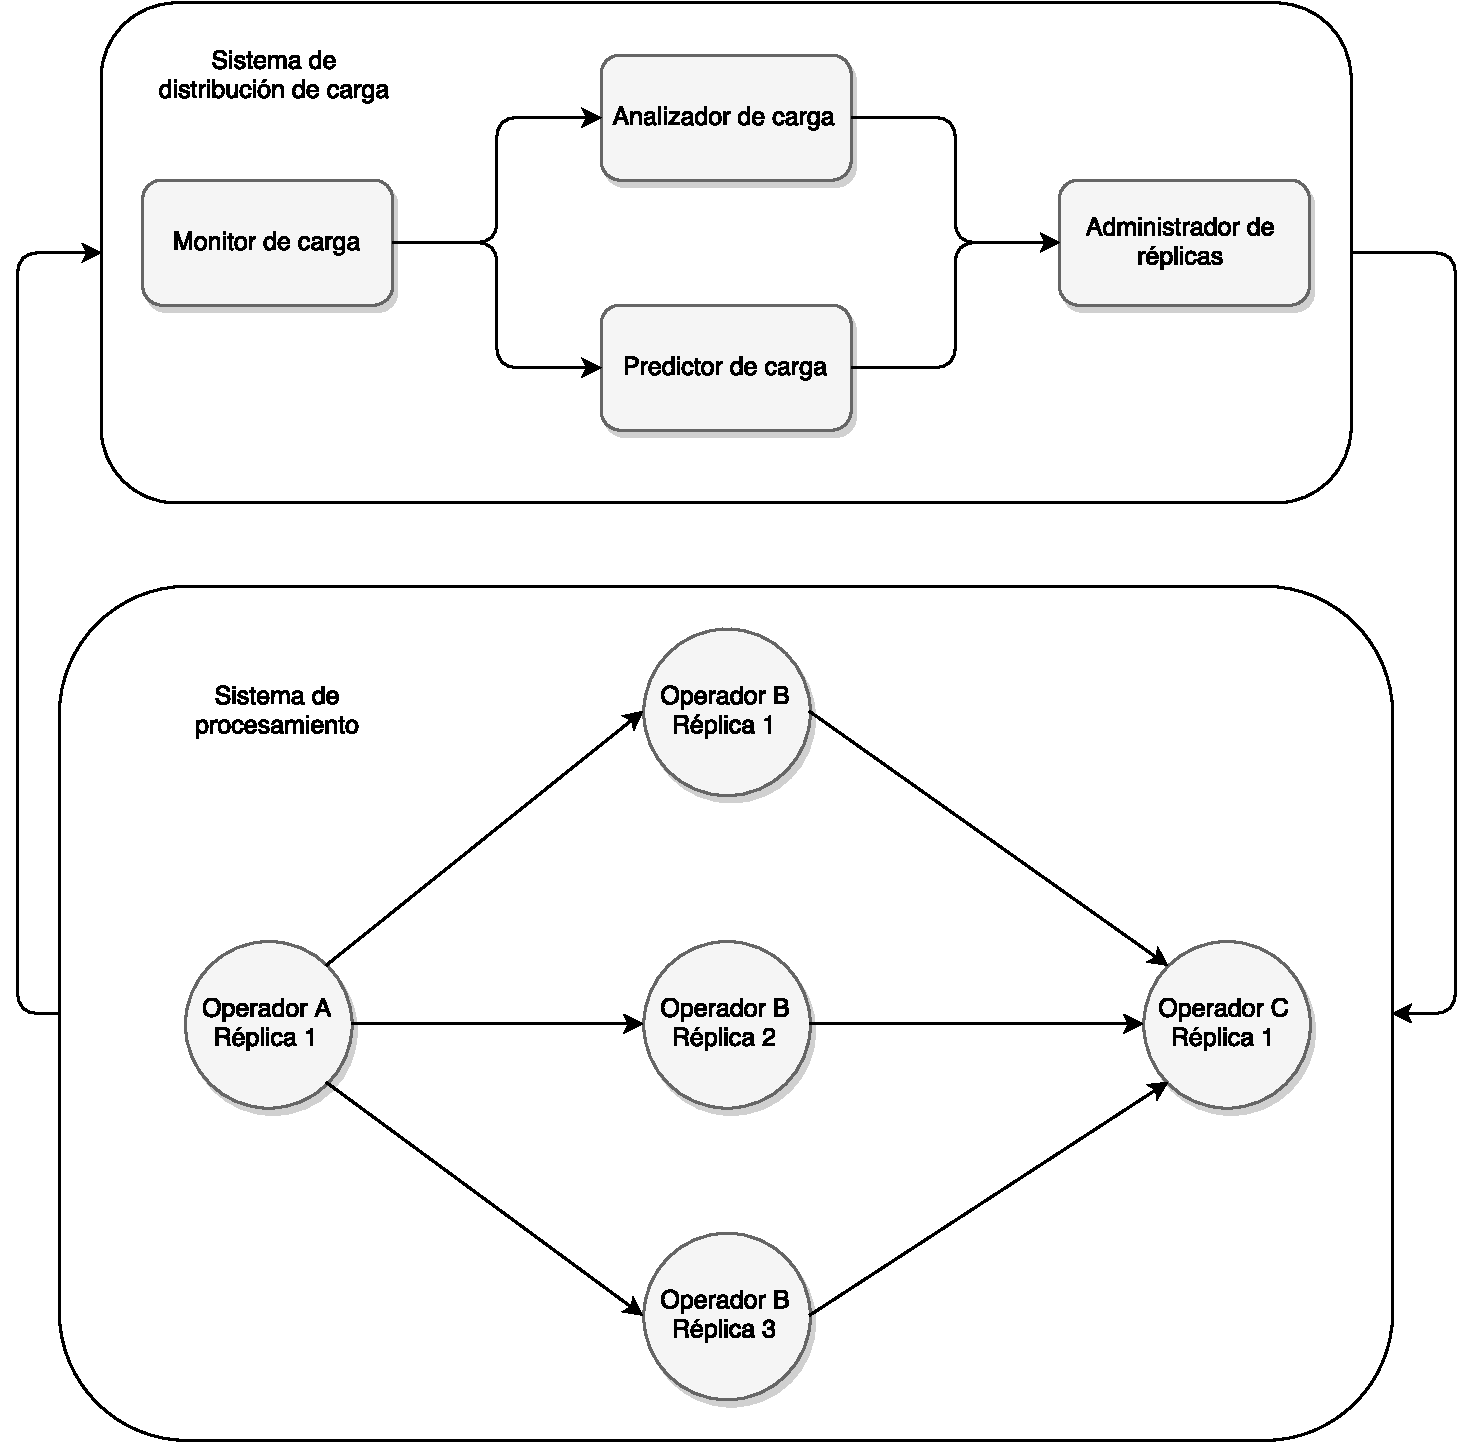
\includegraphics[scale=0.5]{images/Diagrama.pdf}
  \caption[Estructura del modelo el\'astico.]{Estructura del modelo el\'astico.\\Fuente: Elaboraci\'on propia.}
  \label{fig:componentesSistemas}
\end{figure}

A continuaci\'on se describe de manera resumida cada uno de los siguientes m\'odulos, los cuales posteriormente son explicados con mayor profundidad:

\paragraph{Monitor de carga:} est\'a encargado de recolectar las estad\'isticas del sistema, tanto para el algoritmo reactivo, como para el historial del algoritmo predictivo.

\paragraph{Analizador de carga:} analiza la cantidad de carga de un operador en un per\'iodo de tiempo determinado seg\'un el algoritmo reactivo, y respecto a esto indica el estado del operador,  el cual puede ser ocioso, estable o inestable.

\paragraph{Predictor de carga:} es el m\'odulo del algoritmo predictivo que analiza la historia de un operador en una ventana de tiempo determinada, utilizando como muestra la tasa de rendimiento del operador, para posteriormente realizar una cadena de Markov seg\'un las variaciones del sistema. Posteriormente, para la predicci\'on de la carga del operador, se calcula la distribuci\'on estacionaria \citep{Papoulis1984}, el cual entrega la probabilidad que el operador se encuentre en cada uno de los posibles estados.

\paragraph{Administrador de r\'eplicas:} se encarga de determinar cu\'al es el algoritmo a utilizar en cada per\'iodo de tiempo, ya sea reactivo o predictivo, y la administraci\'on de las r\'eplicas utilizando como entrada la informaci\'on prevista por el analizador y predictor de carga.

%\vspace*{0.5cm}

\section{Recolecci\'on de los datos}
%Como se hab\'ia mencionado anteriormente, el monitor de carga est\'a encargado de recolectar la tasa de rendimiento de cada uno de los operadores, tanto del historial como los datos en el momento. Para esto, se consider\'o una ventana de tiempo de 1 segundo para la recolecci\'on del historial, y 5 segundos para el an\'alisis del operador en el momento.

Como se hab\'ia mencionado anteriormente, el monitor de carga est\'a encargado de recolectar los datos necesarios para el funcionamiento del modelo el\'astico, tanto el historial para el algoritmo predictivo, como la tasa de rendimiento para el algoritmo reactivo. La recolecci\'on de muestras se realiza en una ventana de tiempo $T_m$.

%Cada muestra est\'a compuesta por la tasa de rendimiento del operador en ese per\'iodo, la cual es utilizada por el algoritmo reactivo para determinar el estado del operador seg\'un los umbrales propuestos. Dentro de las consideraciones realizadas para la recolecci\'on de datos para el algoritmo reactivo, est\'a el considerar que la tasa de procesamiento ($\mu$) es homog\'enea con el transcurso del tiempo, considerando que los datos procesados son homog\'eneos, por lo tanto, se considera un valor promedio de la tasa de procesamiento seg\'un los primeros datos procesados.

\normalsize{Cada muestra est\'a compuesta por la tasa de llegada y la tasa de procesamiento del operador, la cual es utilizada tanto por el algoritmo reactivo como predictivo. Por parte del algoritmo reactivo, se considera el promedio de las tasas de llegada y servicio en la \'ultima ventana de tiempo $T_r$. En cambio, para el algoritmo predictivo, se considera las muestras obtenidas en la \'ultima ventana de tiempo $T_p$.

Dentro de las consideraciones realizadas para la recolecci\'on de datos, dentro de las consideraciones est\'a que la tasa de procesamiento del operador es homog\'enea. Por lo tanto, se realiza un \textit{benchmark} de la tasa de procesamiento del operador al inicio de la ejecuci\'on del sistema con las primeras muestras obtenidas, de tal manera de obtener el valor que se utiliza para el c\'alculo de la tasa de rendimiento.}

%De esta manera, se espera que existan $n$ muestras para que se ejecute el algoritmo predictivo, por lo que existe una ventana de tiempo $T_p$ entre cada ejecuci\'on del algoritmo. %La cantidad de muestras fue determinado seg\'un la literatura, debido que se considera un n\'umero apropiado para realizar una predicci\'on del operador \citep{GongGW10}.

%Analizar con m\'as detalle el tema de mu, porque quiz\'a es err\'oneo lo descrito aqu\'is
%\normalsize{Por otra parte, para la obtenci\'on de muestras para el algoritmo reactivo, se consideran muestras obtenidas en per\'iodos de $T_r$.} La muestra est\'a compuesta por la tasa de rendimiento del operador en ese per\'iodo, la cual es utilizada por el algoritmo reactivo para determinar el estado del operador seg\'un los umbrales propuestos. Dentro de las consideraciones realizadas para la recolecci\'on de datos para el algoritmo reactivo, est\'a el considerar que la tasa de procesamiento ($\mu$) es homog\'enea con el transcurso del tiempo, considerando que los datos procesados son homog\'eneos, por lo tanto, se considera un valor promedio de la tasa de procesamiento seg\'un los primeros datos procesados. 

%Cabe destacar que cuando el algoritmo predictivo se ejecuta, no es necesaria la recolecci\'on de los datos del per\'iodo, debido que el algoritmo reactivo no se ejecuta en el mismo per\'iodo que el predictivo. S\'olo la recolecci\'on del historial es realizada en todo momento, dado que \'estas son guardadas para posteriormente ser analizadas por el algoritmo predictivo. Debido a los algoritmos utilizados, es que se ha considerado ventanas de tiempo de un segundo para la recolecci\'on de muestras para el an\'alisis predictivo, y $T_p$ para el an\'alisis reactivo.

\section{Algoritmo reactivo}

%El dise\~no del algoritmo reactivo se basa en el an\'alisis del estado del operador en un per\'iodo determinado, siendo definido su estado por una variable del operador, el cual depende del rango en que se encuentre dado los umbrales que se establecen. Este dise\~no analiza seg\'un la tasa de rendimiento ($\rho$), donde el estado del operador depende del valor que \'este posea seg\'un los par\'ametros del algoritmo.

\normalsize{Este an\'alisis emplea las muestras obtenidas en la \'ultima ventana de tiempo $T_r$, las cuales permiten describir el estado del operador (ocioso, estable o inestable) en dicha ventana de tiempo.}

En el Algoritmo \ref{alg:reactive} se presenta el mecanismo de an\'alisis de estado para un operador dado. Dicho estado est\'a determinado por su tasa de rendimiento, la cual en caso de ser mayor a 1, su estado es inestable, si es menor a 0.5, su estado es ocioso, y en otro caso, significa que est\'a estable. Estos datos posteriormente son considerados por el administrador de r\'eplicas, para una posible modificaci\'on de la cantidad de r\'eplicas seg\'un el comportamiento del operador.

\begin{algorithm}[!ht]
	\caption{Algoritmo reactivo del modelo el\'astico.}
	\label{alg:reactive}
	\begin{algorithmic}[1]
	\REQUIRE Tasa de rendimiento $\rho$ del operador $i$.
	\ENSURE Actual estado $\delta$ del operador $i$.
	\IF {$\rho_i > 1$}
		\RETURN $\phi_i$: ``inestable"
	\ELSIF {$\rho_i < 0.5$}
		\RETURN $\delta_i$: ``ocioso"
	\ELSE
		\RETURN $\delta_i$: ``estable"
	\ENDIF
	\end{algorithmic}
\end{algorithm}

En la Figura \ref{fig:umbrales} se observa el estado de un operador seg\'un la tasa de procesamiento. En los primeros 90 segundos la tasa del operador es mayor al l\'imite superior, lo cual indica que el sistema es inestable, es decir, el operador posee sobrecarga. Posteriormente, en el segundo 50, la tasa de rendimiento empieza a disminuir, ya sea por una optimizaci\'on sobre los recursos l\'ogicos o una disminuci\'on de la tasa de llegada. \normalsize{Por lo que ahora el operador ya no se encuentra sobrecargado (inestable), sino que se encuentra entre el l\'imite inferior y superior, cuyo rango define al operador como un sistema estable hasta el segundo 170, donde se encuentra ocioso, hasta llegar al segundo 230.}

\begin{figure}[ht!]
  \centering
  \captionsetup{justification=centering}
    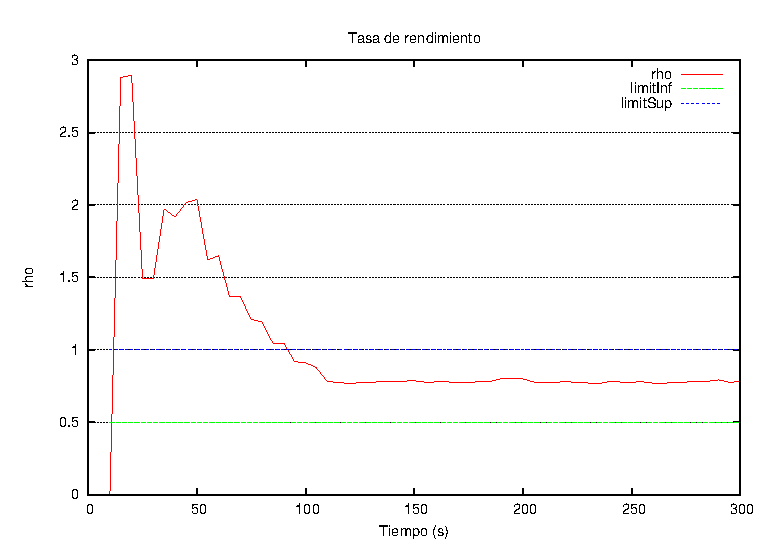
\includegraphics[scale=0.8]{images/Umbrales.eps}
	\caption[Comportamiento de la tasa de procesamiento de un operador.]{Comportamiento de la tasa de procesamiento de un operador. \\ Fuente: Elaboraci\'on propia.}
  \label{fig:umbrales}
\end{figure}


\section{Algoritmo predictivo}
Para la confecci\'on del algoritmo predictivo se ha realizado un an\'alisis seg\'un las cadenas de Markov \citep{ching2006markov}, por lo que se tuvieron que seguir las siguientes etapas:

\begin{itemize}
	\item Definir muestras en tiempos discretos, las cuales cambian con el tiempo seg\'un un proceso estoc\'astico. Las muestras se definieron como la tasa de procesamiento ($\rho$) del operador, la cual dependiendo de su valor, otorgan un estado al operador.
	\item Determinar los estados finitos que se utilizan para la conformaci\'on de la cadena, que son los estados que se puede encontrar el operador: ocioso, estable o inestable.
	\item Obtener una cantidad representativa de muestras para la construcci\'on de la cadena de Markov en el per\'iodo analizado. Estas muestras son independientes entre un per\'iodo y otro, por lo que los valores de la cadena de Markov cambian en cada per\'iodo de tiempo. %Para la implementaci\'on del algoritmo, se ha considerado cien muestras por cada per\'iodo, cuyos intervalos de tiempo son de cien segundos, valor establecido en base al trabajo de \citep{GongGW10}.
\end{itemize}

Tomando las bases anteriores, se ha dise\~nado una cadena de Markov en base a tres posibles estados: ocioso, estable e inestable, como se muestra en la Figura \ref{fig:cadenaMarkovPredictiva}. Cada uno de los estados posee una probabilidad de transici\'on hacia alg\'un estado, cuyas probabilidades est\'an definidas por las muestras obtenidas en el per\'iodo de tiempo analizado.

\begin{figure}[ht!]
  \centering
  \captionsetup{justification=centering}
    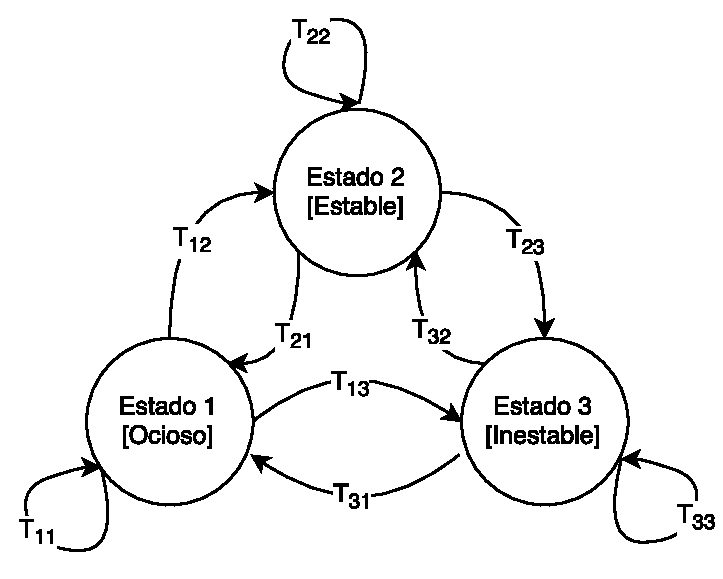
\includegraphics[scale=0.75]{images/CadenaMarkovPredictiva.pdf}
  \caption[Cadena de Markov dado el modelo propuesto del sistema.]{Cadena de Markov dado el modelo propuesto del sistema.\\Fuente: Elaboraci\'on propia.}
  \label{fig:cadenaMarkovPredictiva}
\end{figure}

%Por lo tanto, para cada operador existe una cadena de Markov seg\'un la historia existente en una ventana de tiempo. Para la generaci\'on de esta cadena de Markov, se puede ver en el Ap\'endice \ref{apendice:matrizTransicion} el algoritmo que crea la matriz de transici\'on seg\'un el historial del operador, la cual corresponde a la tasa de rendimiento recolectada cada un segundo en la \'ultima ventana de tiempo del operador analizado. En la Ecuaci\'on \ref{eq:matrizTransicionPredictive} se puede ver la matriz de transici\'on que se obtiene de la cadena de Markov de la Figura \ref{fig:cadenaMarkovPredictiva}, la cual posee una probabilidad de transici\'on desde cada uno de los estado a otro existente.

Por lo tanto, para cada operador se construye una cadena de Markov seg\'un el historial obtenido en la ventana de tiempo $T_p$. Para la conformaci\'on de la cadena de Markov se ha considerado las muestras de la historia de los operadores, por lo que el comportamiento del estado entre una muestra a otra representa una transici\'on, las cuales dan origen a la matriz de transici\'on. En el Anexo \ref{apendice:matrizTransicion} se presenta el algoritmo que se ha empleado para construir esta matriz. En la ecuaci\'on \ref{eq:matrizTransicionPredictive} se muestra la matriz de transici\'on que se obtiene de la cadena de Markov de la Figura \ref{fig:cadenaMarkovPredictiva}.

\begin{equation} \label{eq:matrizTransicionPredictive}
	P =
	\begin{bmatrix}
		T_{1,1} & T_{1,2} & T_{1,3} \\
		T_{2,1} & T_{2,2} & T_{2,3} \\
		T_{3,1} & T_{3,2} & T_{3,3}
	\end{bmatrix}	
\end{equation}

Obtenida la matriz de transici\'on se puede calcular la distribuci\'on estacionaria de la cadena de Markov, la cual indica las probabilidades de que en el futuro el operador est\'e en cada uno de los posibles estados, ya sea ocioso, estable o inestable. Para este c\'alculo se utiliza la ecuaci\'on de Chapman-Kolmog\'orov \citep{Papoulis1984} descrita en la Secci\'on \ref{subsec:cadenaMarkov}.

El Algoritmo \ref{alg:distEstacionaria} describe el c\'alculo de la distribuci\'on estacionaria, cuya entrada es la matriz de transici\'on de un operador del SPS y $upsilon$ que corresponde a la cantidad de transiciones realizadas para obtener la distribuci\'on estacionaria. 

\begin{algorithm}[!t]
	\caption{C\'alculo de la distribuci\'on estacionaria de la cadena de Markov de un operador $i$.}
	\label{alg:distEstacionaria}
	\begin{algorithmic}[1]
	\REQUIRE $P$ Matriz de transici\'on del operador $i$ y $\upsilon$ cantidad de iteraciones deseadas.
	\ENSURE $\Delta$ Distribuci\'on estacionaria de la cadena de Markov del operador $\phi$.
	\STATE $i \leftarrow 1$
	\FOR {$k=0$ a $\upsilon$}
		\STATE $u = randomUniform(0,1)$
		\STATE $\sigma = 0$
		\FOR {$j=1$ a $3$}
			\STATE $\sigma = \sigma + P_{i,j}$
			\IF {$u \leqslant  \sigma$}
				\STATE $\tau_{j}++$
				\STATE $i \leftarrow j$
				\STATE \textbf{break}
			\ENDIF
		\ENDFOR
	\ENDFOR

	\FOR{$k=1$ a $3$}
		\STATE $\Delta_{k} \leftarrow \nicefrac{\tau_{k}}{\upsilon}$
	\ENDFOR	
	
	\RETURN $\Delta$
	
	\end{algorithmic}
\end{algorithm}

%Antes de realizar el c\'alculo, es importante analizar si efectivamente existen transiciones en todos los estados, debido a que existe la posibilidad que no haya una transici\'on a un estado en particular en un per\'iodo de tiempo. Por ejemplo, puede ocurrir que en una ventana de tiempo nunca se ha alcanzado el estado ocioso en el sistema, pero si el estable o inestable. Como el c\'alculo de la distribuci\'on estacionaria requiere un estado de inicio, se ha verificado si efectivamente existe o no el estado, y en caso no existir, el estado de inicio es alguno existente.

\normalsize{Antes de realizar el c\'alculo de la distribuci\'on estacionaria, es importante determinar si la cadena es irreductible y sus estados son recurrentes positivos aperi\'odicos. En caso de ser reductible, se debe determinar la cadena irreductible, y utilizar \'esta para el c\'alculo de la distribuci\'on estacionaria.}

La cantidad de iteraciones $\upsilon$ que debe realizarse para el c\'alculo correspondiente, es un par\'ametro entrada del algoritmo. Es importante destacar que entre mayor es la cantidad de iteraciones, mayor es la precisi\'on del valor predicho. Esto implica a su vez un mayor tiempo de c\'omputo, por lo que en este trabajo se ha considerado un valor medio determinado por pruebas que permitieron medir el costo en tiempo de c\'omputo versus la calidad de los resultados obtenidos.

%se ha considerado un punto medio, de tal manera de lograr un bajo margen de error, pero con bajo costo en el tiempo de ejecuci\'on.

%en este trabajo consideramos un valor medio determinado por pruebas que permitieron medir el costo en tiempo de computo versus la calidad de los resultados obtenidos.

Obtenida la distribuci\'on estacionaria, se procede a analizar las probabilidades obtenidas y como es el comportamiento del operador. Para esto, se ha considerado que las variables aleatorias obtenidas tengan una desviaci\'on est\'andar superior a $\alpha$. El anterior par\'ametro tiene por objetivo reducir la incertidumbre en el momento de seleccionar un estado como posible comportamiento futuro. \normalsize{Por lo tanto, un valor de $\alpha$ adecuado permite establecer una diferencia significativa entre las variables aleatorias al considerar uno de estos estados, disminuyendo el error de la predicci\'on realizada.} En el caso que no supere la desviaci\'on est\'andar, puede ser que dos probabilidades sean muy parecidas y la probabilidad no sea un comportamiento determinante \citep{soong2004fundamentals}. El Algoritmo \ref{alg:predictive} detalla el an\'alisis que se realiza a la distribuci\'on estacionaria, siendo en primer lugar el an\'alisis estad\'istico de las probabilidades, y en segundo lugar la obtenci\'on del estado con mayor valor de las probabilidades, retornando finalmente el estado del operador.

\begin{algorithm}[t]
	\caption{Algoritmo predictivo del modelo el\'astico.}
	\label{alg:predictive}
	\begin{algorithmic}[1]
	\REQUIRE$\Delta$ Distribuci\'on estacionaria de la cadena de Markov del operador $\phi$.
	\ENSURE Futuro estado $\delta^{+}$ de la predicci\'on del operador $i$
	\IF {$\sigma(\Delta_1,\ldots,\Delta_m) > \alpha; m \epsilon [1,3]$} 
		\RETURN $\delta^{+}$: \texttt{max}({$\Delta_1,\ldots,\Delta_m$})

	\ELSE
		\RETURN $\delta^{+}$: ``estable"
	\ENDIF
	\end{algorithmic}
\end{algorithm}

\section{Administraci\'on del sistema}

El \'ultimo componente del modelo es el administrador de r\'eplicas, cuya funci\'on es administrar la cantidad de r\'eplicas en cada uno de los operadores seg\'un los recursos disponibles en el sistema y seg\'un el estado que adopte un operador, ya sea a futuro o en el momento.

%Para esto, se ha dise\~nado un administrador que ejecuta uno de los algoritmos (reactivo o predictivo) seg\'un el per\'iodo del ciclo que se encuentre el sistema. Cada ciclo posee 20 per\'iodos, donde los primeros 19 corresponden al algoritmo reactivo y el \'ultimo corresponde al algoritmo predictivo. Cada per\'iodo posee un intervalo de 5 segundos, de esta manera, cada ciclo tiene un intervalo de 100 segundos, la cantidad necesaria para obtener las muestras para el algoritmo predictivo, suponiendo que cada muestra es obtenida cada 1 segundo.

\normalsize{Para esto, se ha dise\~nado un administrador que ejecuta el algoritmo reactivo en un per\'iodo de $T_r$ y el algoritmo predictivo en un per\'iodo de $T_p$. Cabe destacar, que la ventana de tiempo utilizada para el algoritmo reactivo es menor que la del predictivo, esto debido que uno analiza el comportamiento en el momento y otro a futuro seg\'un la historia.}

En el Algoritmo \ref{alg:administracion} est\'a el procedimiento de administraci\'on, donde primero se analiza qu\'e tipo de algoritmo se debe ejecutar seg\'un el per\'iodo del ciclo. En caso de ejecutarse el m\'odulo predictivo, se analiza el resultado de la predicci\'on, por lo que si el estado es ocioso el sistema disminuye la cantidad de r\'eplicas y si es inestable las aumenta. Como el proceso de predicci\'on se realiza con menor frecuencia y analiza una mayor ventana de tiempo, se ha considerado que se debe modificar una mayor cantidad de r\'eplicas que en el m\'odulo reactivo. Por otra parte, de realizarse el algoritmo reactivo se analiza si existen $\beta$ alertas consecutivas del mismo estado del operador, ya sea ocioso o inestable, y de ser as\'i, realizar una modificaci\'on a la cantidad de r\'eplicas del operador. Adem\'as de cambiar el estado actual del operador a estable, de tal manera de no considerar ese per\'iodo para el pr\'oximo an\'alisis reactivo.

Una de las consideraciones que se han tenido para el dise\~no del administrador, es limitar la cantidad m\'axima de r\'eplicas que pueden realizarse. Esto se debe a que una de las limitantes de este trabajo es que se utiliza solo una m\'aquina, y por ende la cantidad de recursos son limitados, por lo que al aumentar la cantidad de r\'eplicas indefinidamente genera una sobrecarga en los recursos disponibles por parte de la m\'aquina.

\begin{algorithm}[!ht]
	\caption{Administraci\'on de r\'eplicas de un operador $i$ dado su comportamiento en el modelo el\'astico.}
	\label{alg:administracion}
	\begin{algorithmic}[1]
	\REQUIRE Operador $i$ a analizar y $\iota$ la ventana de tiempo del modelo el\'astico.
	\ENSURE Cantidad de r\'eplicas a modificar del operador.	
	\IF {$\iota$ es $T_p$}
		\STATE $\delta_{\iota} \leftarrow AlgoritmoPredictivo(\phi)$
		\IF {$\delta_{\iota}$: ``inestable"}
			\IF {No excede la cantidad m\'axima de r\'eplicas en el sistema}
				\RETURN Crear $\theta$ r\'eplicas del operador $i$
			\ENDIF
		\ELSIF {$\delta_{\iota}$: ``ocioso"}
			\RETURN Remover $\theta$ r\'eplicas del operador $i$
		\ENDIF
	\ELSE[$\iota$ es $T_r$]
		\STATE $\delta_{\iota} \leftarrow AlgoritmoReactivo(\phi)$
		\IF {$\delta_{\iota},\dots,\delta_{\iota-(\beta-1)}$: ``inestable"}
			\IF {No excede la cantidad m\'axima de r\'eplicas en el sistema}
				\STATE $\delta_{\iota} \leftarrow \text{estado estable}$ 
				\RETURN Crear $\omega$ r\'eplica del operador $i$
			\ENDIF
		\ELSIF {$\delta_{\iota},\dots,\delta_{\iota-(\beta-1)}$: ``ocioso"}
			\STATE $\delta_{\iota} \leftarrow \text{estado estable}$ 
			\RETURN Remover $\omega$ r\'eplica del operador $i$
		\ENDIF 
	\ENDIF	
	\end{algorithmic}
\end{algorithm}